\documentclass[25pt,a0paper,landscape,margin=0mm,innermargin=12mm,blockverticalspace=8mm,colspace=10mm,subcolspace=6mm]{tikzposter}

\usepackage[utf8]{inputenc}
\usepackage[T1]{fontenc}
\usepackage[scaled]{helvet}
\renewcommand\familydefault{\sfdefault}
\usepackage{graphicx}
\usepackage{booktabs}
\usepackage{array}
\usepackage{ragged2e}
\usepackage{tikz}
\usetikzlibrary{arrows.meta,positioning,shapes.geometric,calc}
\usepackage{enumitem}

\tikzposterlatexaffectionproofoff
\usetheme{Simple}

\definecolor{mypink1}{rgb}{0.858, 0.188, 0.478}
\definecolor{titlecolor}{RGB}{74, 114, 159}
\definecolor{titledarkcolor}{RGB}{51,102,153}
\definecolor{LightGrey}{RGB}{232, 232, 232}
\definecolor{Grey}{RGB}{222, 223, 225}
\definecolor{DarkerGrey}{RGB}{215,217,219}
\definecolor{FontColor}{RGB}{78,84,89}
\definecolor{Red}{RGB}{204,0,0}
\definecolor{L-lig}{RGB}{25,124,192}
\definecolor{point-lig}{RGB}{54,104,163}
\definecolor{G-lig}{RGB}{62,66,68}
\definecolor{Orange}{RGB}{240,163,10}
\definecolor{Gray}{RGB}{186,200,211}
\definecolor{LightRed}{RGB}{214,98,93}
\definecolor{LightBlue}{RGB}{160,200,217}
\definecolor{LightGreen}{RGB}{130,161,119}
\definecolor{Violet}{RGB}{190,144,252}

\colorlet{blocktitlefgcolor}{point-lig}
\colorlet{blocktitlebgcolor}{Grey}
\colorlet{blockbodyfgcolor}{FontColor}
\colorlet{blockbodybgcolor}{white}
\colorlet{innerblocktitlebgcolor}{L-lig}
\colorlet{innerblocktitlefgcolor}{white}
\colorlet{innerblockbodybgcolor}{LightGrey!55}
\colorlet{notefrcolor}{Red!60}
\colorlet{notefgcolor}{white}
\colorlet{notebgcolor}{Red!60}

\setlist[itemize]{leftmargin=1.15em, itemsep=0.16em, topsep=0.12em}
\setlength{\tabcolsep}{8pt}
\renewcommand{\arraystretch}{1.12}

\newcommand{\metriccard}[3]{%
\begin{minipage}[t]{0.48\linewidth}
\centering
\begin{tikzpicture}
\node[
  draw=#3,
  fill=#3!13,
  rounded corners=8pt,
  line width=1.5pt,
  inner sep=9pt,
  minimum width=0.96\linewidth,
  minimum height=2.85cm,
  align=center
] {\begin{minipage}{0.88\linewidth}\centering
{\color{#3}\bfseries\fontsize{38}{42}\selectfont #1}\par
\vspace{0.14cm}
{\bfseries\large #2}
\end{minipage}};
\end{tikzpicture}
\end{minipage}}

\newcommand{\smallmetric}[3]{%
\begin{tikzpicture}
\node[draw=#3, fill=#3!10, rounded corners=6pt, line width=1pt, inner sep=6pt, minimum width=0.29\linewidth, minimum height=1.7cm, align=center] {%
\begin{minipage}{0.25\linewidth}\centering
{\color{#3}\bfseries\LARGE #1}\par
{\bfseries\small #2}
\end{minipage}};
\end{tikzpicture}}

\newcommand{\metricbar}[4]{%
\textbf{#1} &
\begin{tikzpicture}[baseline=-0.6ex]
\draw[fill=LightGrey, draw=LightGrey, rounded corners=3pt] (0,0) rectangle (5.2,0.30);
\draw[fill=#4, draw=#4, rounded corners=3pt] (0,0) rectangle (#2,0.30);
\end{tikzpicture} &
\textbf{#3}\\[0.24cm]}

\tikzset{
  state/.style={draw=point-lig, fill=LightBlue!22, rounded corners=7pt, line width=1.1pt, align=center, inner sep=5pt, minimum width=3.15cm, minimum height=1.15cm},
  action/.style={draw=LightGreen!80!black, fill=LightGreen!22, rounded corners=7pt, line width=1.1pt, align=center, inner sep=5pt, minimum width=3.15cm, minimum height=1.15cm},
  tool/.style={draw=LightRed!90!black, fill=LightRed!18, rounded corners=7pt, line width=1.1pt, align=center, inner sep=5pt, minimum width=3.15cm, minimum height=1.15cm},
  decision/.style={draw=Violet!80!black, fill=Violet!16, diamond, aspect=2.05, line width=1.1pt, align=center, inner sep=2pt, minimum width=3.1cm},
  arrow/.style={-{Latex[length=2.4mm]}, line width=1.0pt, draw=G-lig}
}

\settitle{
\begin{minipage}[b]{0.96\linewidth}
\vspace{1.2cm}
\hspace{1cm}\color{white}{\Huge\textsc{\textbf{\@title}}\par}
\vspace*{1.2em}
\hspace{1cm}\color{white}{\LARGE \@author\par}
\vspace*{1.0em}
\hspace{1cm}{\Large \@institute}
\vspace{0.5cm}
\end{minipage}}

\definetitlestyle{sampletitle}{
width=1189mm, roundedcorners=0, linewidth=2pt, innersep=15pt,
titletotopverticalspace=0mm, titletoblockverticalspace=22mm
}{\begin{scope}[line width=\titlelinewidth, rounded corners=\titleroundedcorners]\draw[fill=point-lig, color=point-lig]
(\titleposleft,\titleposbottom) rectangle (\titleposright,\titlepostop);
\draw[fill=L-lig, color=L-lig] (\titleposleft,\titleposbottom) rectangle (\titleposleft+34,\titlepostop);
\end{scope}}

\title{\parbox{3050pt}{A MODULAR LLM-BASED CONVERSATIONAL RECOMMENDER FOR EVENT MARKETPLACES}}
\author{Leonardo Matias Candio Orme\~n{o}, Candy Veronica Tenorio Gonzales}
\institute{Universidad de Ingenier\'ia y Tecnolog\'ia (UTEC) \quad | \quad Sin Envolturas event-services marketplace}

\usetitlestyle[]{sampletitle}
\setlength{\columnseprule}{0.4pt}

\begin{document}
\maketitle

\begin{columns}
\column{1}
\begin{subcolumns}

\subcolumn{.24}

\block{\textsc{Motivation}}{
\justifying
Event-marketplace users rarely begin with a neat filter query. They describe an event, a budget, a location, and multiple provider needs that arrive in any order.

\vspace{0.35cm}
\begin{itemize}
\item Manual filters expect users to know the catalog before they know the plan.
\item LLM-only chat can produce fluent but unsupported provider claims.
\item A production marketplace needs provider IDs, live evidence, contact actions, and traceability.
\end{itemize}
}

\block{\textsc{Research Question}}{
\innerblock{Central question}{
What modular architecture lets natural-language event requirements become grounded provider recommendations in a real marketplace, and how reliable is it under live scenario-based evaluation?
}
\vspace{0.35cm}
\textbf{Design thesis:} the LLM interprets and writes; the typed runtime decides when to route, retrieve, persist, recommend, defer, or close.
}

\block{\textsc{Event-Plan-First State}}{
\begin{center}
\begin{tabular}{@{}>{\bfseries}p{0.35\linewidth}p{0.51\linewidth}@{}}
\toprule
Plan fields & event type, date, location, guests, budget, preferences \\
Need fields & category, filters, shortlist, selected providers, status \\
Need states & identified, search-ready, shortlisted, selected, deferred, no results \\
Closure & contact validation, lead creation, partial closure support \\
\bottomrule
\end{tabular}
\end{center}
\vspace{0.1cm}
The event plan is the durable artifact. It lets one conversation manage several provider needs without erasing earlier selections when a new need appears.
}

\block{\textsc{Technical Contributions}}{
\begin{itemize}
\item Channel-agnostic runtime: WhatsApp behavior lives in adapters, not core flow logic.
\item Typed workflow graph: route decisions are auditable state-machine outcomes.
\item Grounded recommendations: provider text is tied to IDs and tool evidence.
\end{itemize}
}

\subcolumn{.26}

\block{\textsc{System Architecture}}{
\begin{center}
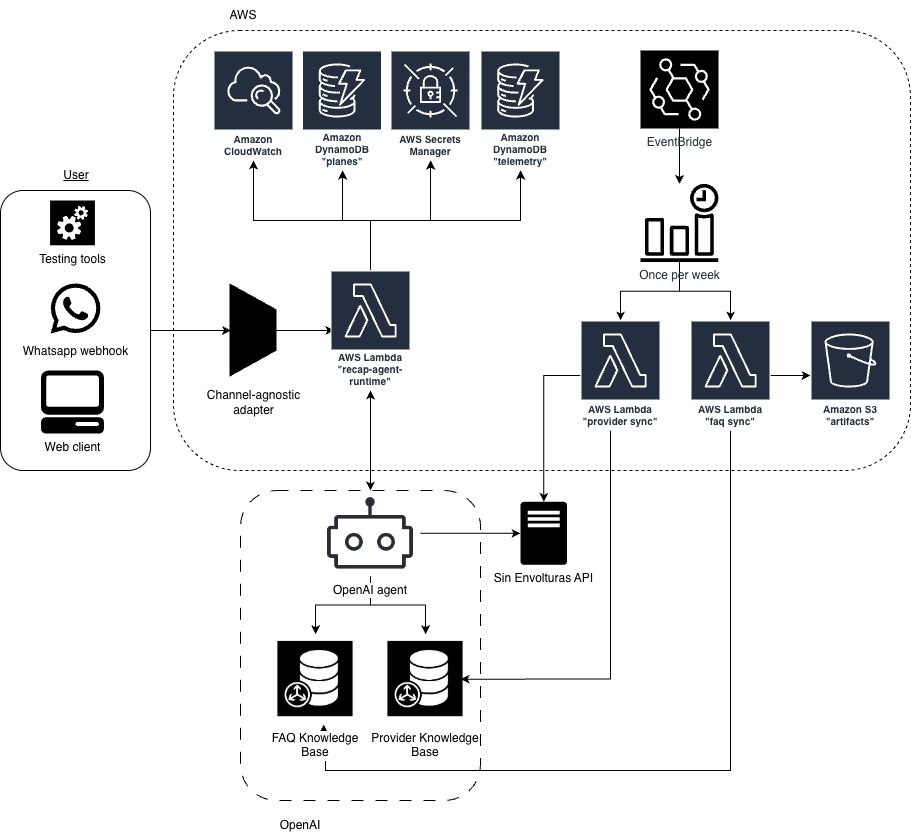
\includegraphics[width=0.82\linewidth]{figures/architecture.png}
\end{center}
\vspace{-0.15cm}
\begin{center}
\begin{tabular}{@{}>{\bfseries}p{0.30\linewidth}p{0.56\linewidth}@{}}
\toprule
Channel & WhatsApp-style adapters, webchat, terminal \\
Runtime & AWS Lambda, typed state, OpenAI Agents SDK \\
Evidence & Sin Envolturas APIs and vector stores \\
Storage & DynamoDB plans and telemetry \\
\bottomrule
\end{tabular}
\end{center}
}

\block{\textsc{Runtime Pattern}}{
\begin{enumerate}[leftmargin=1.2em, itemsep=0.12em, topsep=0.1em]
\item Load the persisted plan for the channel and external user.
\item Extract structured evidence from the Spanish user message.
\item Update the plan and compute a typed node decision.
\item Call only the tools allowed by that node and evidence.
\item Compose a bounded Spanish response and persist telemetry.
\end{enumerate}
\vspace{0.2cm}
Flow decisions come from structured LLM extraction plus typed state-machine evidence. Deterministic code validates invariants and preserves already-established plan state.
}

\block{\textsc{Grounding Strategy}}{
\begin{itemize}
\item Marketplace APIs remain the operational source of truth.
\item Vector stores support semantic retrieval, not free-form claims.
\item Recommendation turns require provider IDs and captured tool evidence.
\end{itemize}
}

\subcolumn{.27}

\block{\textsc{State Diagram}}{
\begin{center}
\resizebox{0.98\linewidth}{!}{%
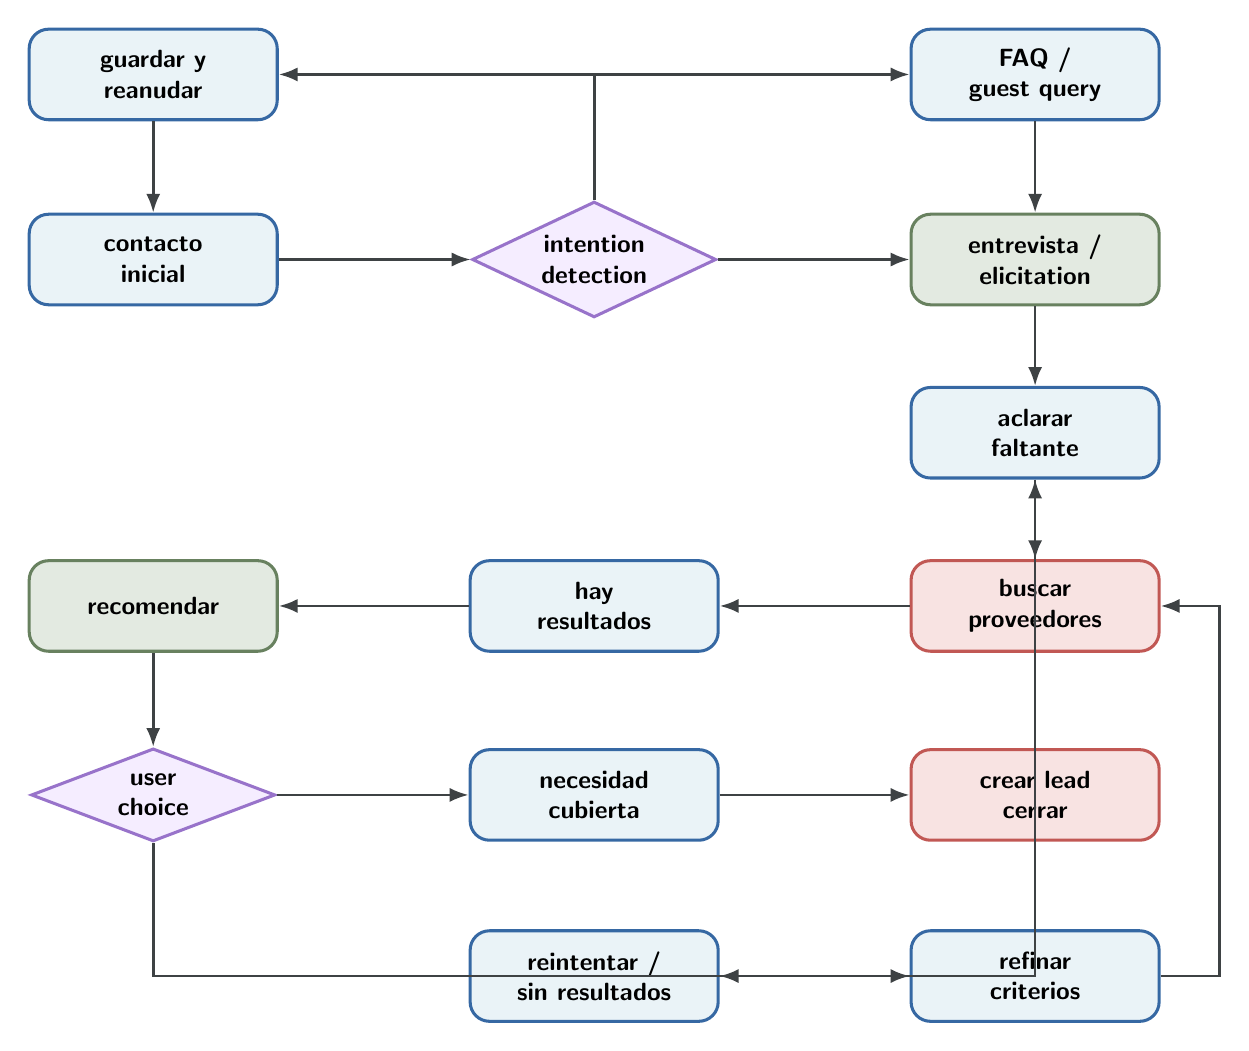
\begin{tikzpicture}[x=1cm,y=1cm, font=\bfseries\small]
\node[state] (start) at (0,5.1) {contacto\\inicial};
\node[decision] (intent) at (5.6,5.1) {intention\\detection};
\node[action] (interview) at (11.2,5.1) {entrevista /\\elicitation};
\node[state] (clarify) at (11.2,2.9) {aclarar\\faltante};
\node[tool] (search) at (11.2,0.7) {buscar\\proveedores};
\node[state] (results) at (5.6,0.7) {hay\\resultados};
\node[action] (recommend) at (0,0.7) {recomendar};
\node[decision] (choice) at (0,-1.7) {user\\choice};
\node[state] (covered) at (5.6,-1.7) {necesidad\\cubierta};
\node[tool] (lead) at (11.2,-1.7) {crear lead\\cerrar};
\node[state] (faq) at (11.2,7.45) {FAQ /\\guest query};
\node[state] (pause) at (0,7.45) {guardar y\\reanudar};
\node[state] (retry) at (5.6,-4.0) {reintentar /\\sin resultados};
\node[state] (refine) at (11.2,-4.0) {refinar\\criterios};

\draw[arrow] (start) -- (intent);
\draw[arrow] (intent) -- (interview);
\draw[arrow] (interview) -- (clarify);
\draw[arrow] (clarify) -- (search);
\draw[arrow] (search) -- (results);
\draw[arrow] (results) -- (recommend);
\draw[arrow] (recommend) -- (choice);
\draw[arrow] (choice) -- (covered);
\draw[arrow] (covered.east) -- ++(0.65,0) |- (lead.west);
\draw[arrow] (intent) |- (faq);
\draw[arrow] (faq) -- (interview);
\draw[arrow] (intent) |- (pause);
\draw[arrow] (pause) -- (start);
\draw[arrow] (search) |- (retry);
\draw[arrow] (retry) -| (clarify);
\draw[arrow] (choice) |- (refine);
\draw[arrow] (refine.east) -- ++(0.75,0) |- (search.east);
\end{tikzpicture}}
\end{center}
\vspace{-0.1cm}
The full implementation defines 26 decision nodes; this diagram compresses them into the main operational routes used by the live study.
}

\block{\textsc{Evaluation Design}}{
\begin{center}
\begin{tabular}{@{}>{\bfseries}p{0.40\linewidth}p{0.45\linewidth}@{}}
\toprule
Conversations & 150 live Lambda runs \\
Scenarios & 50 frozen Spanish scenarios, 3 repetitions \\
Event groups & wedding, birthday, baby shower, corporate, social \\
Route families & recommendation, clarification, multi-need, refinement, selection, pause/resume, closure, FAQ, no-results, recovery \\
Provider snapshot & 182 real Sin Envolturas providers \\
\bottomrule
\end{tabular}
\end{center}
}

\block{\textsc{Recommendation Funnel}}{
\begin{center}
\begin{tabular}{@{}p{0.34\linewidth}p{0.38\linewidth}r@{}}
\metricbar{Need extraction}{5.10}{159/162 = 98.15\%}{LightGreen}
\metricbar{Recommendation after extraction}{3.63}{111/159 = 69.81\%}{Orange}
\metricbar{End-to-end need coverage}{3.56}{111/162 = 68.52\%}{Violet}
\end{tabular}
\end{center}
}

\subcolumn{.23}

\block{\textsc{Headline Results}}{
\metriccard{150}{live conversations}{point-lig}\hfill
\metriccard{88.67\%}{typed completion}{LightGreen}

\vspace{0.45cm}
\metriccard{0}{runtime errors or timeouts}{LightRed}\hfill
\metriccard{99.33\%}{persistence assertions}{Orange}

\vspace{0.45cm}
\metriccard{100\%}{category consistency}{LightBlue}\hfill
\metriccard{100\%}{grounding provenance}{Violet}
}

\block{\textsc{Route Reliability}}{
\begin{center}
\begin{tabular}{@{}p{0.47\linewidth}r@{}}
\toprule
Recommendation & 15/15 \\
Clarification & 15/15 \\
Multi-need planning & 15/15 \\
Refinement & 15/15 \\
Closure & 15/15 \\
Error recovery & 12/15 \\
Pause/resume & 3/15 \\
\bottomrule
\end{tabular}
\end{center}
\vspace{0.15cm}
The Lambda was operationally stable; pause/resume behavior remains the clearest functional weakness.
}

\block{\textsc{Provider Evidence Checks}}{
\begin{center}
\smallmetric{704/704}{category match}{LightGreen}\hfill
\smallmetric{0}{known location mismatches}{LightRed}\hfill
\smallmetric{180/180}{evidence-backed turns}{Violet}
\end{center}
\vspace{0.25cm}
Recommendations are constrained by provider IDs, tool outputs, and structured candidate provenance rather than generated provider descriptions alone.
}

\block{\textsc{Takeaway}}{
\innerblock{Main message}{
Grounded conversational recommendation is not just prompt engineering. A reliable event-marketplace agent needs a bounded LLM, explicit workflow control, persistent state, live provider evidence, and audit-ready telemetry.
}
\vspace{0.35cm}
\textbf{Next steps:} enrich provider metadata, strengthen pause/resume, and compare against manual filters and forms.
}

\end{subcolumns}
\end{columns}

\end{document}
